\documentclass[11pt]{jsarticle}

\usepackage{SPR}

\headerSPR
\begin{document}
	\titleSPR{\number\year}{\number\month}{\number\day}{D2}{吉田 皓太郎}
%%%%%%%%%%%%%%%%%%%%%%%%%%%%%%%%%%%%%%
	\articleSPRabst
		\begin{itemize}
			\item 機械学習を用いたカップ形状の設計支援
			\item 着後形状予測のためのカップの変形解析
		\end{itemize}
		
		
	\articleSPRobj
		\begin{enumerate}
			\item 定性的な機能要求を満たせるようなカップ形状を設計できる
			\item 布の物性とカップのパターンがどのような結びつきを持っているかを調べることができる.
		\end{enumerate}
%%%%%%%%%%%%%%%%%%%%%%%%%%%%%%%%%%%%%%
% 1.前回からのノルマ
	\articleSPRitemsone
		%\begin{enumerate}
		%	\item A
		%\end{enumerate}
		
		\tableofcontents
		
		
%%%%%%%%%%%%%%%%%%%%%%%%%%%%%%%%%%%%%%
%\begin{itemize}
%	\item 新規手法について
%	\item ISFAアウトライン
%\end{itemize}
%%%%%%%%%%%%%%%%%%%%%%%%%%%%%%%%%%%%%%
% 2.具体的な成果
	\articleSPRitemstwo
	\renewcommand{\labelitemi}{$\blacktriangledown$}
	%\renewcommand{\labelitemi}{$\bigcirc$}
	\newcommand{\argmax}{\mathop{\rm arg~max}\limits}
	\newcommand{\argmin}{\mathop{\rm arg~min}\limits}
%%%%%%%%%%%%%%%%%%%%%%%%%%%%%%%%%%%%%
	\section{研究進捗について}
		計算がうまくいかない.調査中
	\section{投稿論文修正}
		\begin{itemize}
			\item 日曜夜にひとしきりまとめたものを送信いたしました.
			\item 結果についてですが,おそらくすべて完璧な状態のものを出すことができなさそうです...なんとか頑張ってみますが,無理な場合はこちらのデータを示します.この場合,誤差について何か触れた方がよろしいでしょうか
		\end{itemize}
	\bfig[H]
		\centering
		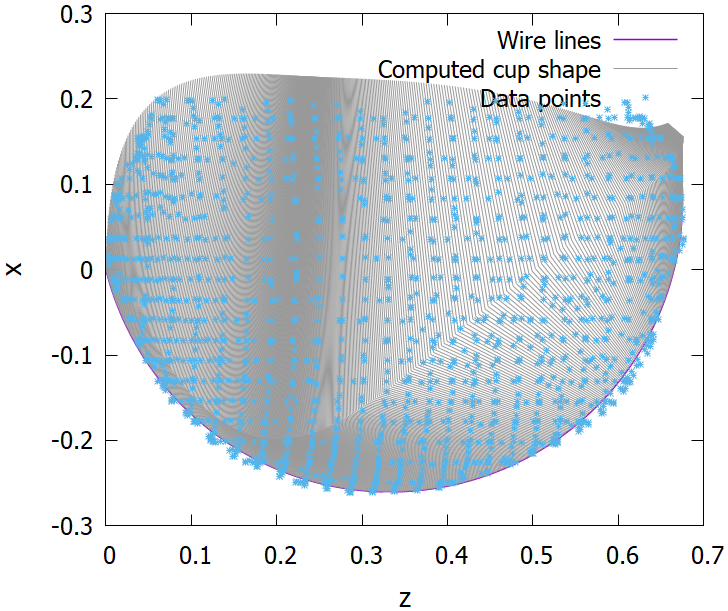
\includegraphics[width=0.6\columnwidth]{./figure/Measure/ObtainedRidgeLinefromz-x.png}
		\caption{z-x}
	\efig
	\bfig[H]
	\centering
	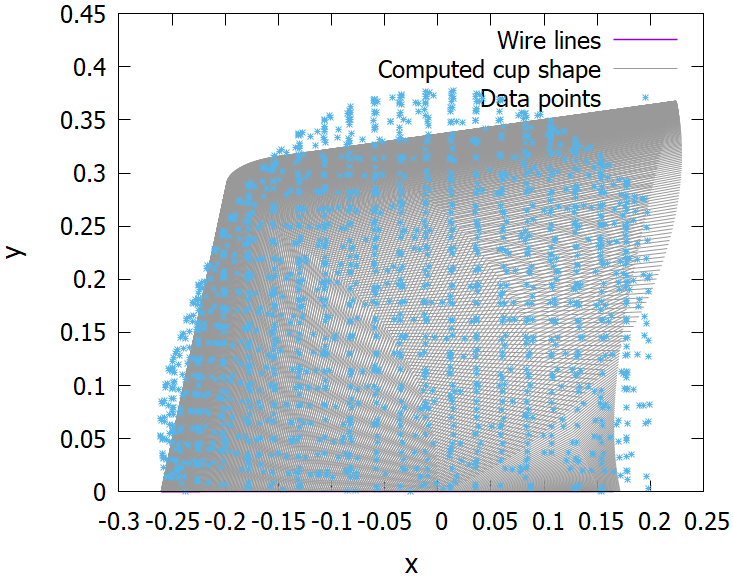
\includegraphics[width=0.6\columnwidth]{./figure/Measure/ObtainedRidgeLinefromx-y.png}
	\caption{x-y}
	\efig
	
	\bfig[H]
	\centering
	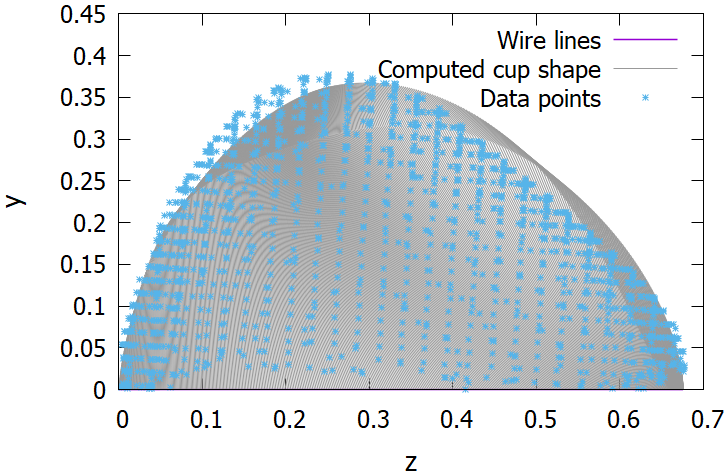
\includegraphics[width=0.6\columnwidth]{./figure/Measure/ObtainedRidgeLinefromz-y.png}
	\caption{z-y}
	\efig
	
	\bfig[H]
		\centering
		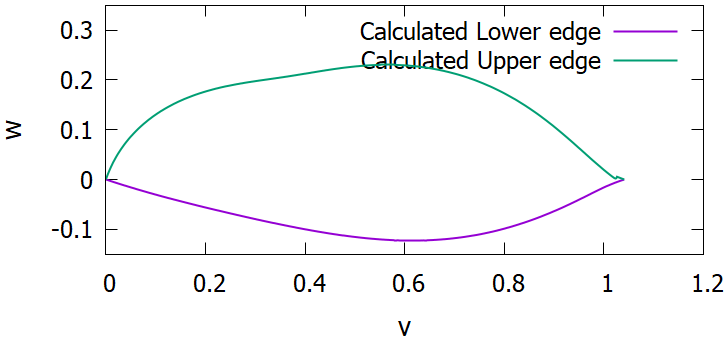
\includegraphics[width=0.6\columnwidth]{./figure/Measure/ObtainedPatternL.png}
		\caption{L}
	\efig
	
	\bfig[H]
	\centering
	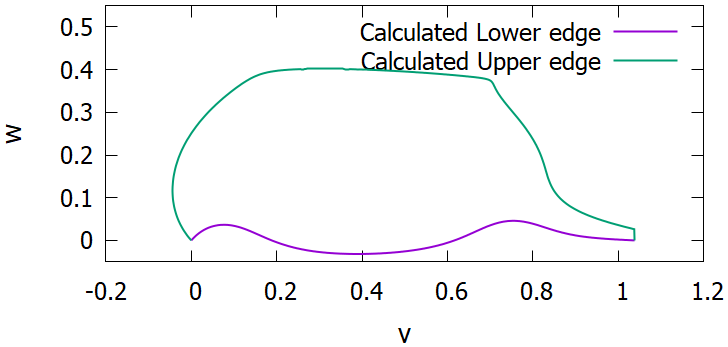
\includegraphics[width=0.6\columnwidth]{./figure/Measure/ObtainedPatternU.png}
	\caption{U}
	\efig
	\section{参考)査読者コメント}
		\begin{itemize}
			\item Reviewer1
			
			This paper proposes a method to design the two-dimensional shapes of patterns of two-piece brassiere cup. Mathematical modeling for shape fitting is well considered. I could not confirm the quality of modeling and its implementation with the current manuscript, therefore I recommend major revision.  The detailed formulation is potentially valuable for some readers, but it is too abstract and limited to specific situations. I could not understand how well the mathematical formulas cover the actual shape of the breast. To solve the problem, I recommend the major revision for this manuscript. 
			
			\begin{itemize}
				\item Detailed error analysis for more practical shapes 
				
				▼The current manuscript presents the results for only two primitive shapes and does not provide a quantitative evaluation of the results. I would like the authors to present quantitative results for the shapes that more closely resembles actual chest.
				
				▼The authors can use an appropriate dataset of medical images, or human body shape models for 3D modeling software such as Unity or Shade. The quantitative fitting results for at least 10 or so shapes will be necessary. Of course, it is a condition for acceptance of a paper that the method is accurate enough to confirm its validity.
				
				\item Discussion on the limitation 
				
				▼Even if the human body shape is obtained, it is not obvious where the brassiere should cover from and to. Identifying anatomical features from a surface mesh model is a difficult problem in itself. How much coverage one wants should also depend on personal feeling. I would like the authors to add some additional discussions on how to think about these issues from the point of view of real-world applications.
			\end{itemize}
			\item Reviewer2
			
			ブラジャーの設計のために,点群にフィットするように可展面を最適化するとのことですが,Conclusionの章に書いてある"From the proposed method can design the cup shape with manifest the function. As a result, Our proposed method will be useful for efficient design of a two-piece brassiere cup." というのは主張が過多であるように見受けられます.本論文では手法の評価として(1)球状の点群にフィットさせたもの,(2)可展面上の点群にフィットさせたものを使って評価しています.しかしながら(1)球面の点群は実際の胸の形状と大きく異なる,また(2)可展面の点群にフィットできたからといって胸の形状にフィットできるかどうかは分からない,などの問題があります.論文の方向性は間違ってはいないと思うのですが,手法の評価に明らかな欠陥があり,論文の主張が正しくないと思われるので不採録を推薦させて頂きます.
			\begin{itemize}
				\item ページ2-4の可展面の章ですが,多くの議論は既に微分幾何の教科書で取り扱っているレベルの話だと思うので,何か教科書や既存研究などの文献を引用して,どこまでが既存の手法で,どこまでが著者らのオリジナルの手法であるのかを線引きして下さい.
				\item ページ4-6のOptimizationの章ですが,どのように2つのカーブをパラメータ化しているのかが分かりませんでした.カーブのパラメータ化ができないと最適化ができないように思います.読んでも分からなかったので,明記して下さい.
			\end{itemize}
		\end{itemize}
	\newpage
\vspace{10cm}
%%%%%%%%%%%%%%%%%%%%%%%%%%%%%%%%%%%%%%
% 3.達成できなかったこととその問題点
	%\articleSPRthree
	
%%%%%%%%%%%%%%%%%%%%%%%%%%%%%%%%%%%%%%

\vspace{14cm}
%%%%%%%%%%%%%%%%%%%%%%%%%%%%%%%%%%%%%%
	\articleSPRfour
	\articleSPRfive
\end{document}
